\section{Results}
\label{sec:results}

\subsection{RQ1: Structural Break Detection (H-E1)}

PELT detects a single structural break at $\mathbf{\text{paper\_count}^* = 39}$ (breakpoint\_idx $= 8$, BIC penalty $= 4.32$).

\begin{table}[h]
\centering
\caption{H-E1 Primary Results.}
\label{tab:he1}
\begin{tabular}{llll}
\toprule
Metric & Value & Gate Threshold & Status \\
\midrule
Permutation $p$-value & 0.035 & $< 0.05$ & PASS \\
paper\_count$^*$ & 39 & $\in [10, 120]$ & PASS \\
Piecewise $F$-test $p$-value & 0.0021 & (corroborative) & Strong \\
Bootstrap CI (95\%) & [38, 69.5] & --- & --- \\
$n_{\text{bkps}}$ detected & 1 & $\geq 1$ & PASS \\
\bottomrule
\end{tabular}
\end{table}

The permutation test asks: if paper\_count labels were randomly shuffled, how often would PELT place a breakpoint at or before index 8? Only 3.5\% of 1000 permutations do so (Figure~\ref{fig:permutation}). The piecewise $F$-test independently confirms: a two-segment model explains data significantly better than a single linear model ($F=6.46$, $p=0.0021$). Two fundamentally different tests --- randomization and model comparison --- converge on the same structural break.

Figure~\ref{fig:scatter} (CoV scatter with breakpoint marker) makes the regime separation visually apparent: benchmarks left of paper\_count$=39$ show substantially wider spread than those to the right. Figure~\ref{fig:residual} (residual series) reinforces this with explicit pre/post shading.

\textbf{OLS trend note:} The global OLS trend is weakly positive ($\rho = +0.137$, $R^2=0.019$), a reversal from the $\rho=-0.28$ anchor from prior analysis. One plausible explanation is that dataset composition changed between snapshots ($N=111 \to N=115$): newly added benchmarks with high paper\_count and high CoV would locally increase the aggregate trend slope. We do not have per-snapshot benchmark identities to verify this directly; the reversal is acknowledged as an unresolved sensitivity (see \S\ref{sec:limitations} L3). Importantly, PELT operates on OLS residuals --- after removing whatever linear trend exists --- making the structural break finding robust to trend direction regardless of the reversal's cause.

\begin{figure}[h]
\centering
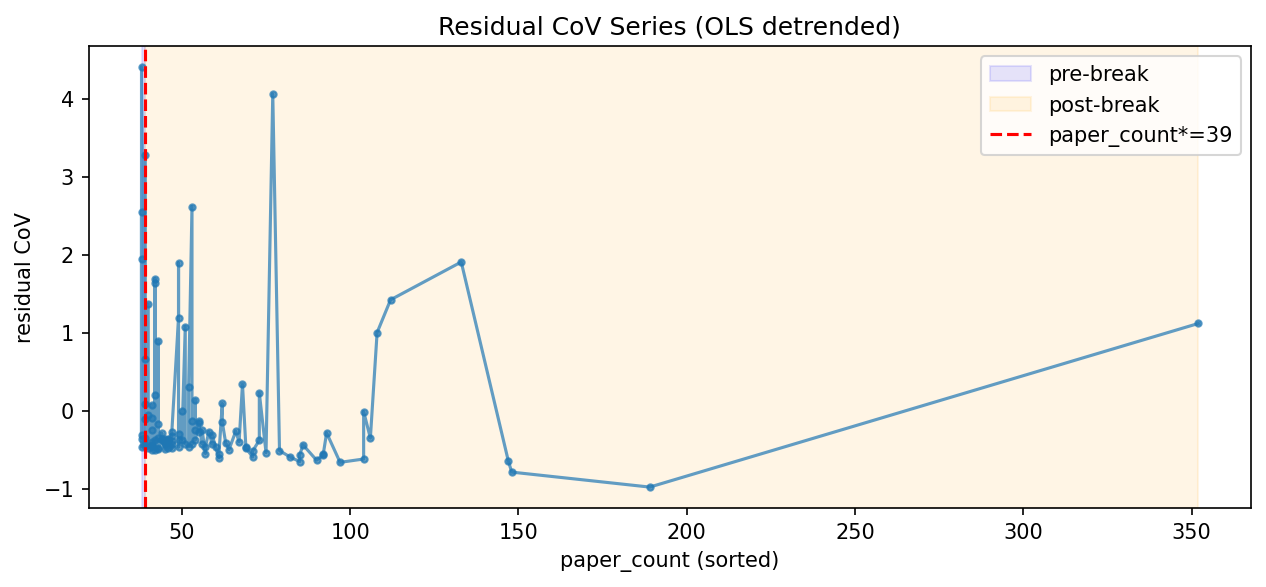
\includegraphics[width=0.48\textwidth]{figures/fig3_residual_series.png}
\caption{Residual CoV series with pre/post regime shading. The structural break at paper\_count$^*=39$ separates the high-variance exploration phase (left) from the low-variance saturation phase (right).}
\label{fig:residual}
\end{figure}

\begin{figure}[h]
\centering
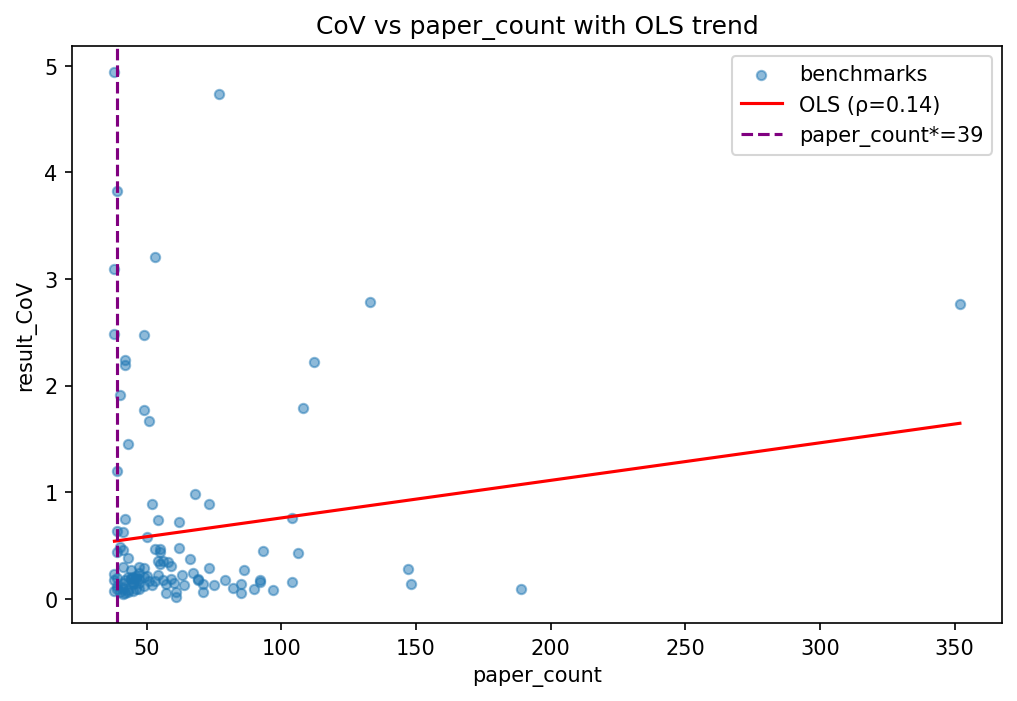
\includegraphics[width=0.48\textwidth]{figures/fig2_cov_scatter.png}
\caption{CoV vs.\ paper\_count scatter with breakpoint marker. Benchmarks left of paper\_count$=39$ exhibit substantially wider spread.}
\label{fig:scatter}
\end{figure}

\begin{figure}[h]
\centering
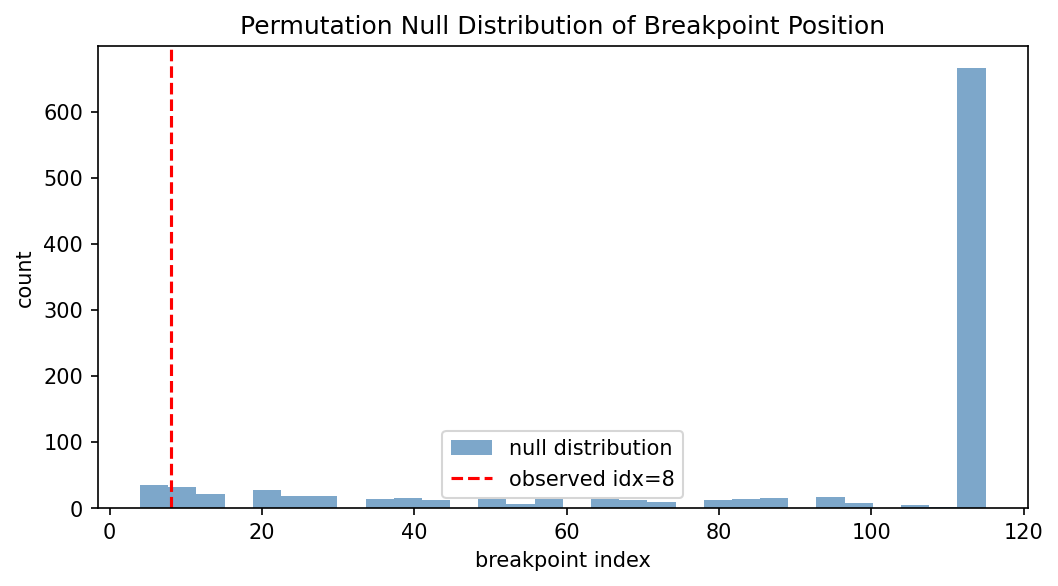
\includegraphics[width=0.48\textwidth]{figures/fig4_permutation_null.png}
\caption{Permutation null distribution with observed breakpoint marked. Only 3.5\% of permutations place a breakpoint at or before index 8 ($p=0.035$).}
\label{fig:permutation}
\end{figure}

\subsection{RQ2: Exploration Regime Confirmation (H-M1)}

\begin{table}[h]
\centering
\caption{H-M1 Results --- Exploration Regime.}
\label{tab:hm1}
\begin{tabular}{llll}
\toprule
Metric & Value & Gate Threshold & Status \\
\midrule
Global variance & 0.911 & (baseline) & --- \\
Pre-segment variance & 3.475 & $>$ global & PASS \\
Variance ratio (pre/global) & 3.814 & $> 1.0$ & PASS \\
$F$-test one-tailed $p$-value & 0.0009 & $< 0.10$ & PASS \\
Pre-segment mean residual CoV & $+0.873$ & $> 0$ & --- \\
\bottomrule
\end{tabular}
\end{table}

The pre-breakpoint segment ($n=8$) is nearly $\mathbf{4\times}$ \textbf{more variable} than the global baseline ($F$-test $p=0.0009$). Figure~\ref{fig:varbar} (variance bar chart) shows the pre-segment bar towers over the global baseline. The positive mean residual CoV ($+0.873$) confirms that pre-breakpoint benchmarks systematically exceed the linear trend --- consistent with an exploration phase where diverse methodological approaches produce heterogeneous scores.

\begin{figure}[h]
\centering
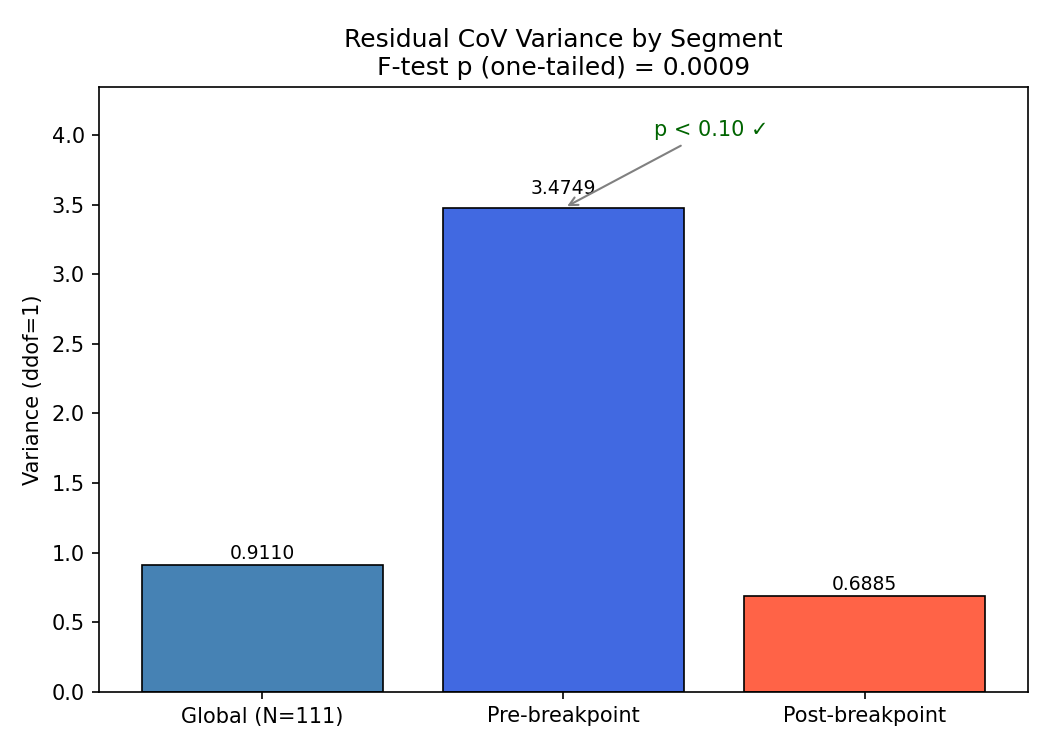
\includegraphics[width=0.48\textwidth]{figures/fig01_variance_bar.png}
\caption{Pre-segment vs.\ global baseline variance bar chart. The pre-segment variance ($3.475$) is $3.81\times$ the global baseline ($0.911$).}
\label{fig:varbar}
\end{figure}

\subsection{RQ3: Saturation Compression (H-M2 and H-M3)}

\begin{table}[h]
\centering
\caption{H-M2 Results --- Saturation Compression.}
\label{tab:hm2}
\begin{tabular}{llll}
\toprule
Metric & Value & Gate Threshold & Status \\
\midrule
Pre-segment variance & 3.475 & (reference) & --- \\
Post-segment variance & 0.688 & $<$ pre & PASS \\
Variance ratio (post/pre) & 0.1981 & $< 1.0$ & PASS \\
Brown-Forsythe $p$-value & 0.0099 & $< 0.05$ & PASS \\
Piecewise $F$-test $p$-value & 0.0022 & --- & Significant \\
\bottomrule
\end{tabular}
\end{table}

\textit{(Note: The piecewise $F$-test $p$-value here, $p=0.0022$, differs slightly from the H-E1 value in Table~\ref{tab:he1}, $p=0.0021$. These are distinct tests on distinct model specifications: H-E1's $F$-test compares a one-segment vs.\ two-segment linear model on the full residual CoV series to confirm break existence; H-M2's $F$-test compares pre vs.\ post segment fits within the variance-comparison model. Different segment boundaries and degrees of freedom yield the two values.)}

An \textbf{80\% variance reduction} (ratio$=0.1981$) after paper\_count$^*=39$ operationalizes ``saturation'' as a measurable quantity. Figure~\ref{fig:varbars2} (variance bars) shows the collapse across pre-segment, post-segment, and global baseline. Figure~\ref{fig:boxplots} (boxplots) makes the distributional difference concrete: the post-segment distribution is markedly tighter.

\begin{figure}[h]
\centering
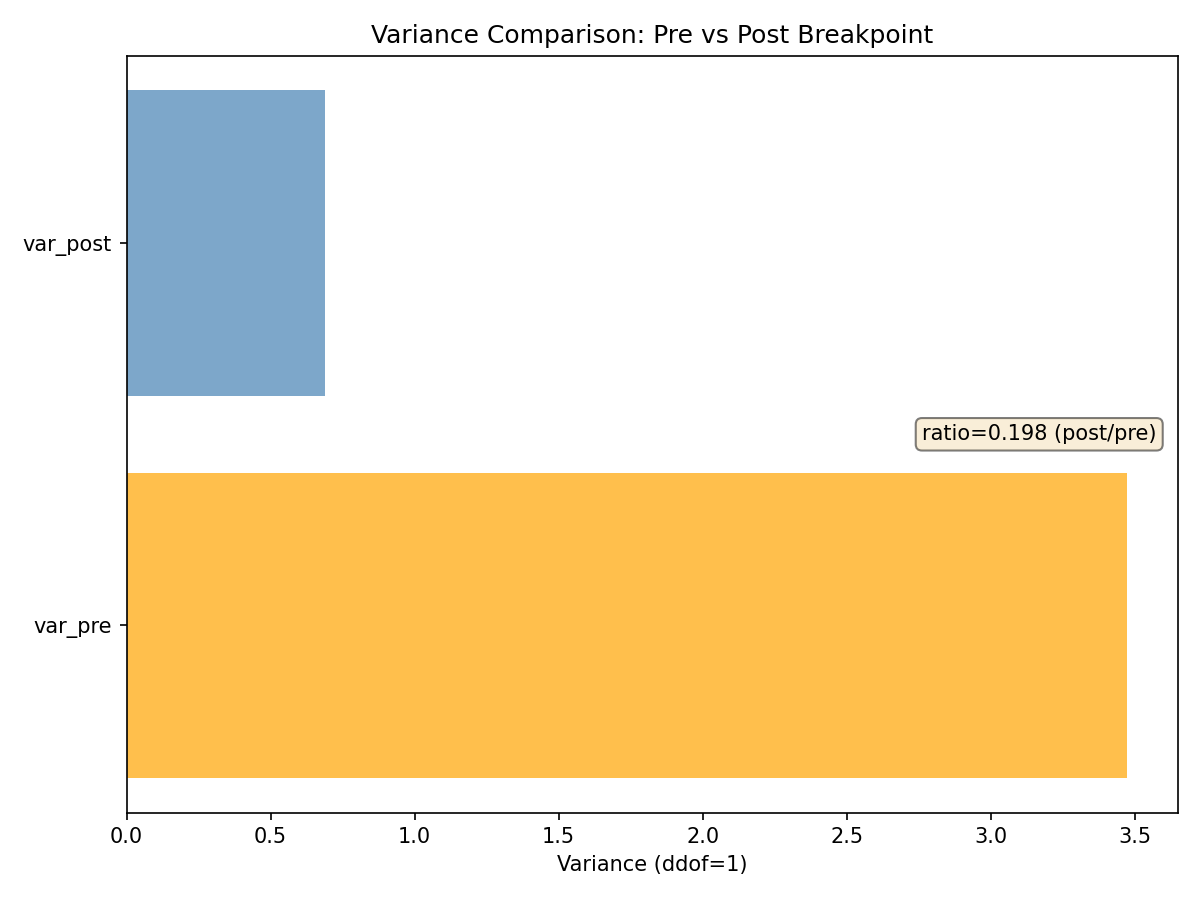
\includegraphics[width=0.48\textwidth]{figures/variance_bars.png}
\caption{Variance magnitude: pre-segment, post-segment, and global baseline. The post-segment variance ($0.688$) is $0.20\times$ the pre-segment ($3.475$).}
\label{fig:varbars2}
\end{figure}

\begin{figure}[h]
\centering
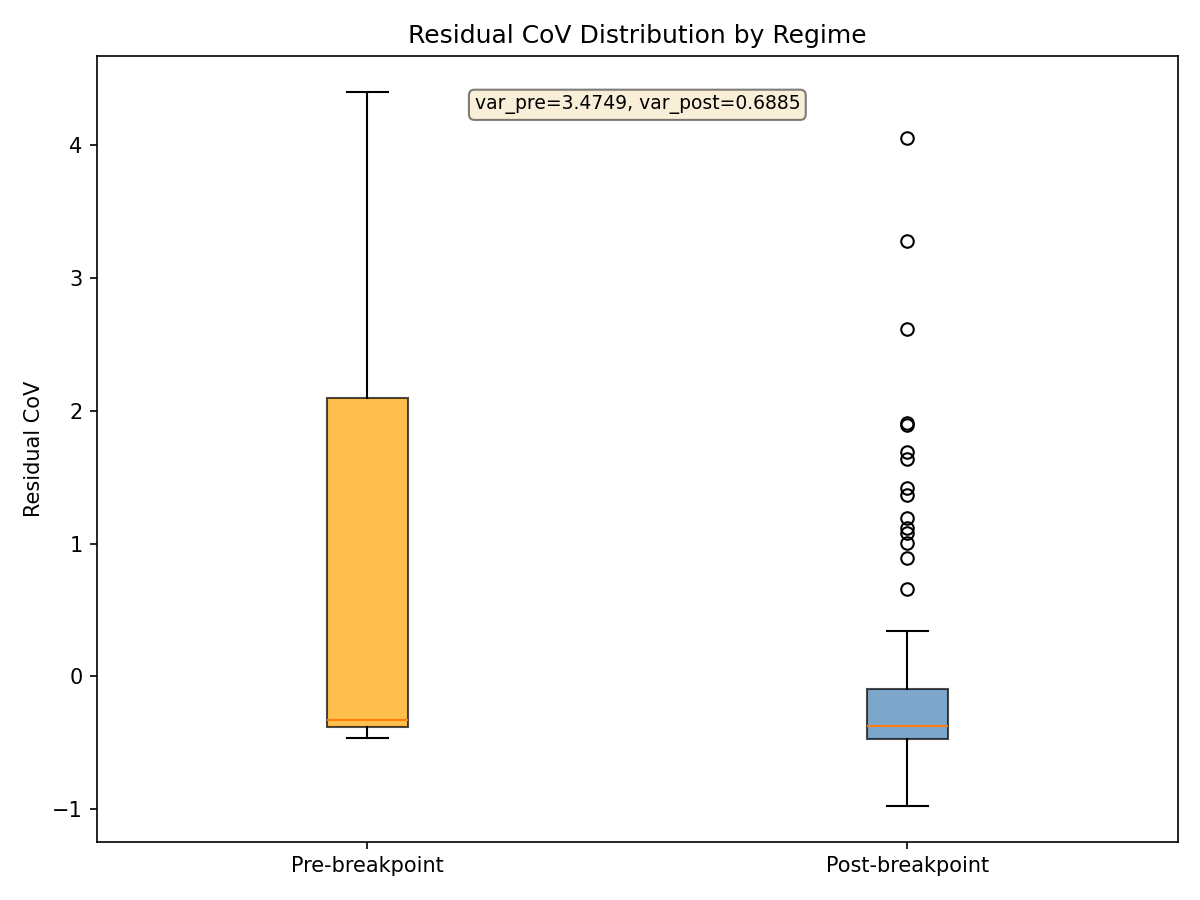
\includegraphics[width=0.48\textwidth]{figures/boxplots_pre_post.png}
\caption{Pre vs.\ post residual CoV boxplots. The post-segment distribution is markedly tighter, visualizing the 80\% variance collapse.}
\label{fig:boxplots}
\end{figure}

\begin{table}[h]
\centering
\caption{H-M3 Directional Metrics.}
\label{tab:hm3}
\begin{tabular}{lll}
\toprule
Metric & Result & Status \\
\midrule
M1: Skewness direction (skew\_post $<$ skew\_pre) & skew\_post$=2.71 >$ skew\_pre$=1.18$ & FAIL \\
M2: Lower-tail (p10\_post $<$ p10\_pre) & p10\_post$=-0.568 <$ p10\_pre$=-0.435$ & \textbf{PASS} \\
M3: Permutation test on skewness difference & $p=0.51$ & FAIL \\
M4: Mann-Whitney dominance pre $>$ post & $p=0.058$ & \textbf{PASS} \\
\bottomrule
\end{tabular}
\end{table}

M2 and M4 pass the SHOULD\_WORK gate ($\geq$2/4). Figure~\ref{fig:histogram} shows the histogram overlay with p10 markers. M1 and M3 fail because moment-based estimates on $n_{\text{pre}}=8$ have high sampling variance --- a known limitation (Section~\ref{sec:limitations}).

\subsection{Cross-Experiment Convergence}

\begin{table}[h]
\centering
\caption{Cross-Experiment Summary.}
\label{tab:summary}
\begin{tabular}{lllp{2.5cm}}
\toprule
Hypothesis & Gate & Key Evidence & Confidence \\
\midrule
H-E1: Break at paper\_count$^*=39$ & MUST\_WORK: PASS & Permutation $p=0.035$, $F$ $p=0.0021$ & HIGH \\
H-M1: Pre-regime variance $3.81\times$ global & MUST\_WORK: PASS & $F$-test $p=0.0009$ & HIGH \\
H-M2: Post-regime variance $5\times$ lower & MUST\_WORK: PASS & BF $p=0.0099$, ratio$=0.1981$ & HIGH \\
H-M3: Post-regime directional concentration & SHOULD\_WORK: PASS (2/4) & 2/4 metrics pass at $p<0.10$ (M2+M4) & MEDIUM \\
\bottomrule
\end{tabular}
\end{table}

Three independently designed experiments converge on the same two-regime narrative --- substantially reducing the probability of a Type I error.

\subsection{Bootstrap Uncertainty}

Figure~\ref{fig:bootstrap} shows the bootstrap distribution of paper\_count$^*$ (1000 resamples): 95\% CI $= [38, 69.5]$, width$=31.5$. This width reflects the small pre-segment ($n_{\text{pre}}=8$); when 8 observations are resampled with replacement, some bootstrap samples shift the estimate rightward. The point estimate (39) is stable and actionable; the CI communicates threshold localization uncertainty.

\begin{figure}[h]
\centering
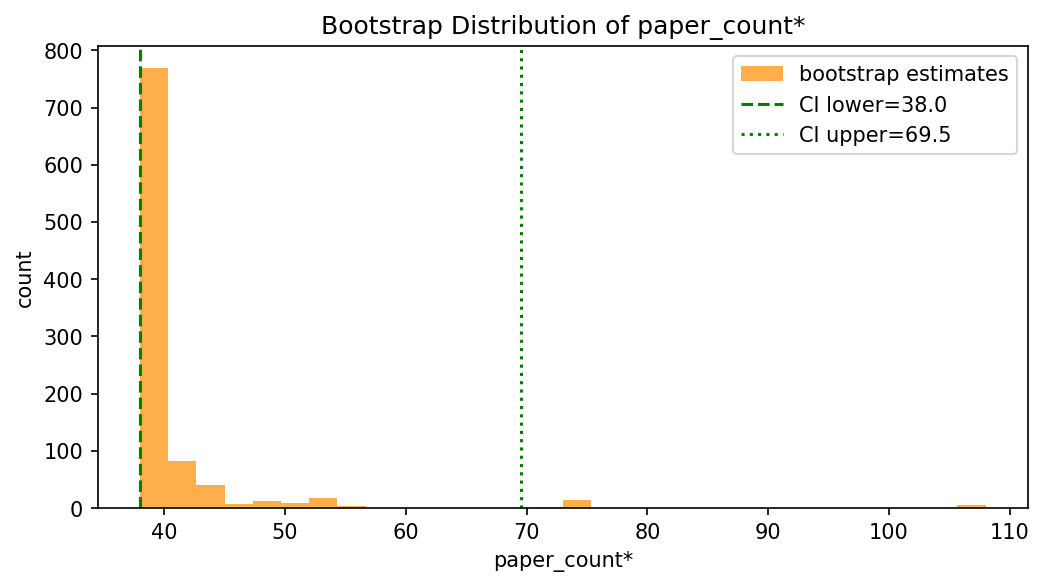
\includegraphics[width=0.48\textwidth]{figures/fig5_bootstrap_ci.png}
\caption{Bootstrap distribution of paper\_count$^*$ (1000 resamples). 95\% CI $= [38, 69.5]$.}
\label{fig:bootstrap}
\end{figure}

\begin{figure}[h]
\centering
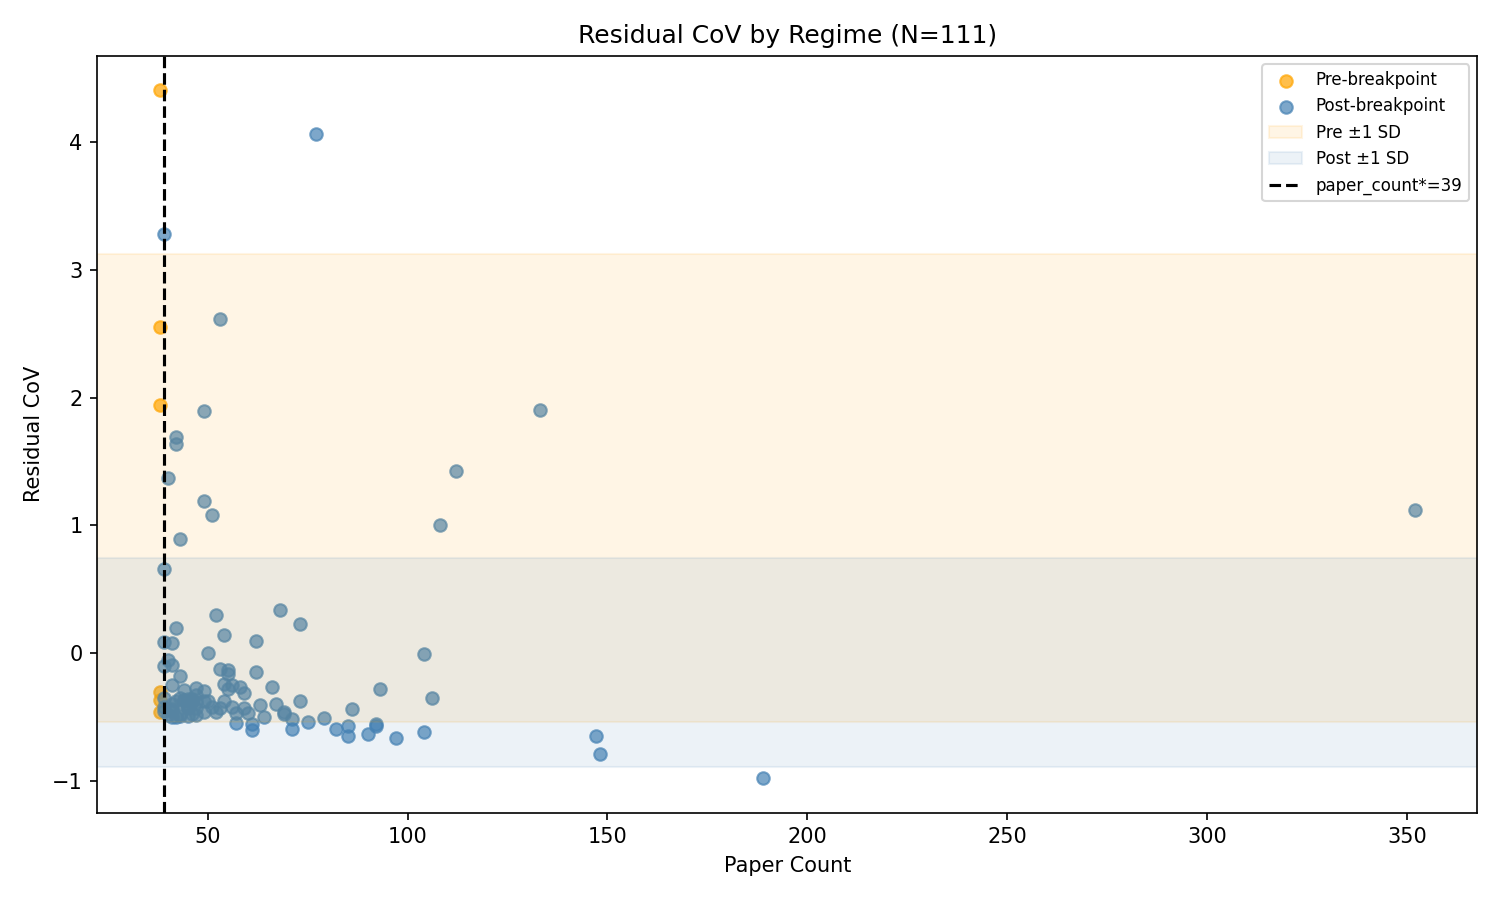
\includegraphics[width=0.48\textwidth]{figures/scatter_regime.png}
\caption{Residual CoV scatter colored by regime. The two-regime structure is visually apparent.}
\label{fig:regime}
\end{figure}

\begin{figure}[h]
\centering
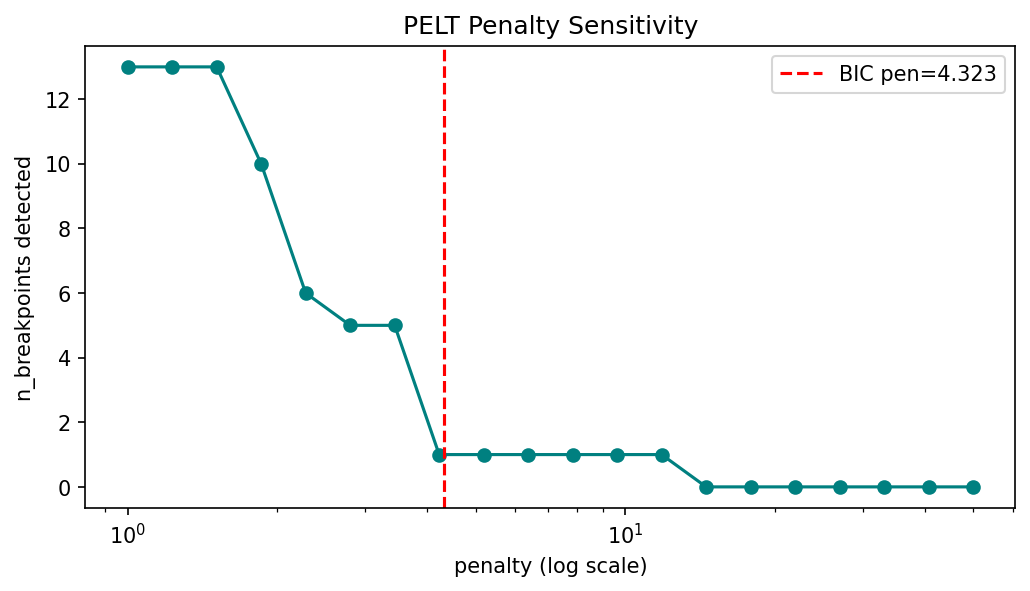
\includegraphics[width=0.48\textwidth]{figures/fig6_penalty_sensitivity.png}
\caption{PELT penalty sensitivity: number of detected breakpoints vs.\ penalty. A single breakpoint is detected robustly across the relevant penalty range.}
\label{fig:penalty}
\end{figure}

\begin{figure}[h]
\centering
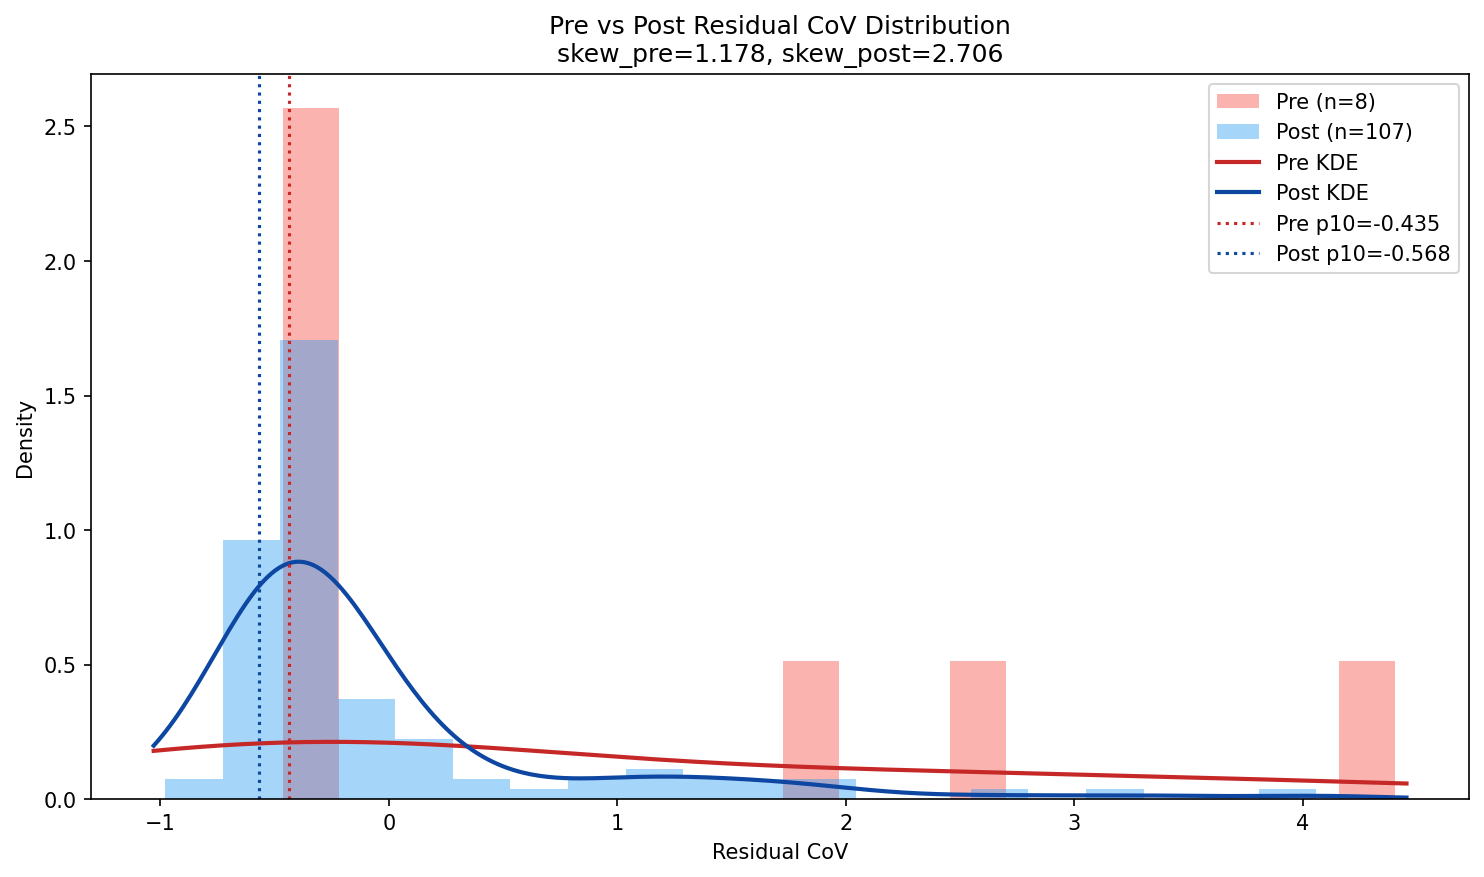
\includegraphics[width=0.48\textwidth]{figures/histogram_overlay.png}
\caption{Pre/post KDE + histogram with p10 markers. M2 (lower-tail) passes: p10\_post $< $ p10\_pre.}
\label{fig:histogram}
\end{figure}
